\documentclass[a4paper,12pt]{scrartcl}
\usepackage[utf8]{inputenc}
\usepackage[ngerman]{babel}
\usepackage[T1]{fontenc}
\usepackage{amsmath}
\usepackage{stmaryrd}
\usepackage{wasysym}
\usepackage{lmodern}
\usepackage{graphicx}
\usepackage{paralist}
\usepackage{upgreek}
\usepackage{subfigure}
\usepackage{tipa}
\usepackage{amssymb}
\usepackage{gensymb}
\usepackage{dsfont}
\usepackage{fancyhdr}

%\title{Abgabe 1}
%\author{Rafael Heid, Julian Deinert, Sabrina Buczko Gruppe\\ 6 und 7}
%\date{Abgabe am 24.10.16}

\gdef\blatt{FGI-2 Aufgabenblatt 01}

\title{\blatt}
\date{Gruppe 06}
\author{Sabrina Buczko 6663234, Julian Deinert 6535880, Rafael Heid 6704828}


\pagestyle{fancy}
\fancyhf{}
\fancyhead[L]{\blatt}
\fancyhead[R]{Buczko, Deinert, Heid}
\fancyfoot[C]{\thepage}

\begin{document}
\maketitle
\newpage
\setcounter{section}{0}

\section{}
\setcounter{subsection}{3}
\subsection{}
\subsubsection{}
Endlich bedeutet, dass wir eine endliche Menge an Zuständen sowie ein endlich langes Wort zur Eingabe haben.
\subsubsection{}
Unsere akzeptierte Sprache muss mind. das Zeichen b enthalten. Es müssen gleich viele a's und c's im Wort enthalten sein, damit wir im Endzustand landen.\\
%sprich b oder abc oder aabcc oder aaabccc ....
$L(A)=\{a^{n}bc^{n} | n\in \mathds{N_{0}}\}$
\subsubsection{}
Wir beweisen mit Hilfe des Pumping Lemmas, dass $L(A)$ nicht regulär ist.\\
Angenommen $L$ wäre regulär. Dann gilt das Pumping Lemma für $L$. Sei $k$ die Zahl aus dem Pumping Lemma. Betrachten wir das Wort $z=a^kbc^k$. Wegen $|a^k| = |c^k|$ gilt $z \in L$ und $|z|\geq k$. Somit gilt das Pumping Lemma und es gibt für $z$ eine Zerlegung in $uvw$ mit $|uv|\leq k$, $|v|> 0$ und $\forall i\in \mathbb{N}_0.\, u\cdot v^i\cdot w \in L$. Wir zeigen nun, dass jede Zerlegung von $z$ in $uvw$, die die ersten beiden Bedingungen erfüllt, die dritte nicht erfüllt und das Pumping Lemma somit doch nicht gilt. Da $z$ mit $a^k$ beginnt ist $uv \in \{a\}^*$ wegen $|v|> 0$ gilt sogar $v \in \{a\}^+$. Ferner gibt es ein $j$ mit $1 \leq j \leq k$ derart, dass  $v = a^j$ ist. Betrachten wir nun $uv^2w = a^{k+j}bc^k$ dann gilt $k+j < k$ wegen $j \geq 1$ und somit $uvw \notin L$. Im Widerspruch zum Pumping Lemma ist $L$ also nicht regulär. 
%Zur hilfe: https://github.com/weristspokey/Uni/blob/master/fgi/fgi1_l3.pdf
\subsubsection{}
Die zugehörige Grammatik lautet:\\
$S\rightarrow b | aSc$\\
Wir starten in unserem Startzustand S und können mit der Kante b direkt in den Endzustand gelangen. Man kann aber auch einen Weg über Kante a, Kante b und dann Kante c gehen zum Endzustand. Dies kann immer mehr erweitert werden, und somit sind immer gleich viele a's und c's sowie nur ein b im Wort enthalten. Demnach gilt L(G)=L(A).
\subsubsection{}
$A_{n}$ ist die Schnittmenge aus allen Wörtern aus L(A) die eine Länge n haben. \\
Im Fall \textbf{L(B)} ist n=5. Also ist das Wort nur fünf Zeichen lang. Das einzige akzeptierte Wort aus L(A) das fünf Zeichen hat ist aabcc.\\
Im Fall \textbf{L(C)} ist n=4. Unser Automat A akzeptiert allerdings keine Wörter die eine gerade Anzahl am Eingabesymbole haben, da wir immer eine gleiche Anzahl an a's und c's haben und diese somit immer gerade ist. Dann kommt aber noch unser b dazu, weshalb jedes von A akzeptierte Wort ungerade ist. Daher kann kein Automat mit $L(C)=A_{4}$ angegeben werden, außer einer der nur die leere Menge akzeptiert.
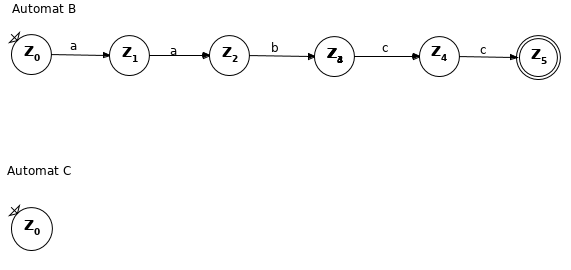
\includegraphics[scale=0.5]{145.png}
 
\subsection{}
\subsubsection{}
Das Verfahren besteht wie in den Präsenzaufgaben zunächst darin, aus dem NFA mittels der Potenzautomatenkonstruktion einen DFA zu machen. Dann vervollständigen wir den Automaten, fügen also noch fehlende Kanten hinzu die in einen Fehlzustand führen. Wenn alle Zustände Endzustände sind, dann gilt $L(A)=\sum^{*}$, da somit alle Wörter akzeptiert werden denn nach jedem Übergang gelangt man in einen Endzustand.
\subsubsection{}
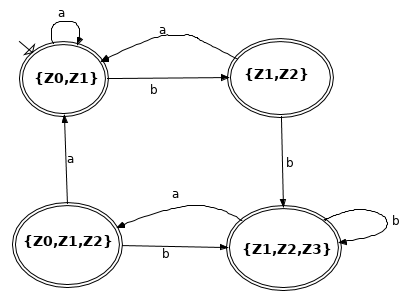
\includegraphics[scale=0.5]{152.png}\\
Wir konstruieren einen Potenzautomaten. Da es von jedem Zustand eine a und eine b Kante gibt, müssen wir keine Kanten hinzufügen. Alle Zustände sind Endzustände. Somit ist es egal welches Wort wir eingeben, das Wort wird immer akzeptiert. Somit gilt für diesen Automaten $L(A)=\sum^{*}$.
\subsubsection{}
Unser Verfahren terminiert, da es sich um einen endlichen Automaten handelt. Daher muss er auch nach endlichen Schritten terminieren. Es ist korrekt, da es prüft ob $L(A)=\sum^{*}$ gilt also alle Wörter akzeptiert werden. Da jeder Zustand ein Endzustand ist, kann der Automat bei keinem Wort aus $\{a,b\}$ blockieren. Und da aus jedem Zustand eine a und eine b Kante führt, kann das Wort beliebig (aber endlich) lang sein.
\subsubsection{}
Es kann der 1.Schritt weggelassen werden, da wir bereits einen DFA haben und ihn nicht mittels Potenzautomatenkonstruktion in einen DFA umwandeln müssen. Ansonsten bleibt das Verfahren gleich, da sich nichts ändert, außer das statt einzelnen Zeichen an den Kanten auch ganze Wörter als Übergänge gelten. Dies hat aber keinen Einfluss auf das Prüfen des Universalitätsproblems.
\end{document}
